%================================
% note-setup-borderless.tex
% fenglielie@qq.com 2025-07-10
%================================
\documentclass{article}
\usepackage{amsmath,amsthm,amsfonts,amssymb}
\usepackage{mathtools}
\usepackage{mathrsfs}
\usepackage{bm}
\usepackage{extarrows}
\usepackage[a4paper, margin=1in]{geometry}
\usepackage{float}
\usepackage{indentfirst}
\usepackage{anyfontsize}
\usepackage{booktabs,multirow,multicol}
\usepackage[shortlabels,inline]{enumitem}
\usepackage{appendix}

\usepackage[dvipsnames]{xcolor}
\usepackage{graphicx}
\graphicspath{
    {./figure/}{./figures/}{./image/}{./images/}{./graphic/}{./graphics/}{./picture/}{./pictures/}
}
\usepackage{subcaption}

\usepackage[ruled,linesnumbered,noline]{algorithm2e}
\usepackage{listings}
\lstdefinestyle{simpleStyle}{
    basicstyle=\ttfamily\small,
    breaklines=true,
    keywordstyle=\color{blue},
    identifierstyle=\color{black},
    stringstyle=\color{violet},
    commentstyle=\color[RGB]{34,139,34},
    showstringspaces=false,
    numbers=left,
    numbersep=2em,
    numberstyle=\footnotesize,
    frame=single,
    framesep=1em,
}
\lstset{style=simpleStyle}

\usepackage[colorlinks=true,linkcolor=,urlcolor=magenta,citecolor=violet]{hyperref}

\renewcommand*{\proofname}{\normalfont\bfseries Proof}

\usepackage{thmtools}

%% define environments

\declaretheorem[style=plain, name=Theorem, numbered=yes, numberwithin=section]{theorem}
\declaretheorem[style=plain, name=Theorem, numbered=no]{theorem*}

\declaretheorem[style=plain, name=Proposition, numbered=yes, sibling=theorem]{proposition}
\declaretheorem[style=plain, name=Proposition, numbered=no]{proposition*}

\declaretheorem[style=plain, name=Corollary, numbered=yes, sibling=theorem]{corollary}
\declaretheorem[style=plain, name=Corollary, numbered=no]{corollary*}

\declaretheorem[style=plain, name=Lemma, numbered=yes, sibling=theorem]{lemma}
\declaretheorem[style=plain, name=Lemma, numbered=no]{lemma*}

\declaretheorem[style=plain, name=Claim, numbered=yes, sibling=theorem]{claim}
\declaretheorem[style=plain, name=Claim, numbered=no]{claim*}

\declaretheorem[style=definition, name=Definition, numbered=yes, numberwithin=section]{definition}
\declaretheorem[style=definition, name=Definition, numbered=no]{definition*}

\declaretheorem[style=definition, name=Example, numbered=yes, numberwithin=section]{example}
\declaretheorem[style=definition, name=Example, numbered=no]{example*}

\declaretheorem[style=definition, name=Problem, numbered=yes, numberwithin=section]{problem}
\declaretheorem[style=definition, name=Problem, numbered=no]{problem*}

\declaretheorem[style=remark, name=Remark, numbered=yes, numberwithin=section]{remark}
\declaretheorem[style=remark, name=Remark, numbered=no]{remark*}

\declaretheorem[style=remark, name=Note, numbered=yes, numberwithin=section]{note}
\declaretheorem[style=remark, name=Note, numbered=no]{note*}

\declaretheoremstyle[headfont=\bfseries, bodyfont=\normalfont, spaceabove=3pt, spacebelow=3pt, qed=\ensuremath{\square}]{solutionstyle}

\declaretheorem[style=solutionstyle, name=Solution, numbered=yes, numberwithin=section]{solution}
\declaretheorem[style=solutionstyle, name=Solution, numbered=no]{solution*}

\usepackage[most]{tcolorbox}

\newcommand{\newtcbenvironment}[2]{
    \tcolorboxenvironment{#1}{#2, enhanced, breakable, sharp corners, boxrule=0pt, colframe=white}
    \tcolorboxenvironment{#1*}{#2, enhanced, breakable, rounded corners, boxrule=0pt, colframe=white}
}

%% define styles

\newtcbenvironment{theorem}{colframe=RoyalPurple, colback=RoyalPurple!8}
\newtcbenvironment{proposition}{colframe=RoyalPurple, colback=RoyalPurple!8}
\newtcbenvironment{corollary}{colframe=NavyBlue, colback=SkyBlue!8}
\newtcbenvironment{lemma}{colframe=NavyBlue, colback=SkyBlue!8}
\newtcbenvironment{claim}{colframe=NavyBlue, colback=SkyBlue!8}

\newtcbenvironment{definition}{colframe=ForestGreen, colback=ForestGreen!5}
\newtcbenvironment{example}{colframe=RawSienna, colback=RawSienna!5}
\newtcbenvironment{problem}{colframe=WildStrawberry!30, colback=WildStrawberry!5}

%Exercise Environment
\newtheorem*{exercise}{Exercise}

\title{MAT4033 Differential Geometry}
\author{Zihan Ke}

\begin{document}
\maketitle
\newpage
\tableofcontents
\newpage
\section*{Foreward}

\newpage
\section*{Introduction}
\noindent In this course we study curves and surfaces in $\mathbb{R^3}$

What are we interested in?
\begin{itemize}
    \item How we decribe a curve?
    \\ use the parametrization: $\alpha:I \to \mathbb{R}^3 $
    \item How much information can we get from $\alpha$?
    \\ length, curvature, torsion
    \item If we know the curvature of a curve of evrey point, can we describe the curve?
    \item Some "global" problems: Suppose we have a closed curve in $\mathbb{R}^3$ of a given length, what is the largest possible area bounded by the curve?
    \item How do we describe a surface? More precisely, what kind of surface should we study?
    \item For a regular surface, how can we study the area and curvature of them?
    \item What is the "shortest" between two points of a surface?
    \item What is the relationship between geometry and topology on surfaces? (Gauss-Bonnet Theorem)
\end{itemize}
\newpage
\section{Local Theory of Curves}
\begin{definition}[regular curve]
    $\alpha: [c,d]\to \mathbb{R}^3$ is called a regular curve if $|\alpha'|\neq0$, ($\alpha$ is taken to be differentiable (smooth))
\end{definition}

\begin{proposition}
    Let $\alpha:[c,d]\to \mathbb{R}^3$ be a given curve with partition $P=\{c=t_0<t_1<\cdots <t_n=b\}$. Let $l(\alpha,P):=\sum |\alpha(t_{i+1})-\alpha(t_{i})|$, then we can have \[\int_c^d |\frac{d\alpha}{dt}|dt=\operatorname{sup}\{l(\alpha,P)| \text{P any partition}\}\]
\end{proposition}
\begin{proof}
The proof is straight forward.
\end{proof}

\begin{proposition}[length is invariant under reparametriazation]
   Given a differntiable curve $\alpha:[a,b]\to \mathbb{R}^3$ and a $g:[c,d] \to [a,b] $ with $\beta=\alpha\circ g$, then \[\int_a^b |\frac{d\alpha}{dt}|dt=\int_c^d|\frac{d\beta}{ds}|ds\] 
\end{proposition}
\begin{proof}
    also straight forward, by simple chain rule.
\end{proof}
There are many ways to parametrize the curves. But we always want to pick one such that the \textit{pointers} is unit.
\begin{remark}
    The cusp is not a regular curve since $\alpha'(0)=0$, but we allow self-intersections, in which case a regular curve may have different tangent at the same point.    
\end{remark}

\subsection{Reparametrization}
Consider $\alpha_1(t)=(\cos t,\sin t), \alpha_2(t)=(\cos(2t),\sin(2t))$, both give the same trace with different parameters.
\begin{definition}
    A reparametrizastion of a curve $\alpha:(a,b)\to \mathbb{R}^3 $ is a bijective function $g:(c,d)\to (a,b)$ such that $g$ is $C^{\infty}$ and $g^{-1}$ is $C^1$. Given a raparametrization $g$, one can define a new "curve" $\beta:(c,d)\to \mathbb{R}^3$ by $\beta=\alpha\circ g$
\end{definition}

\begin{example}[nonexample]
    $g(s)=s^3$, we can check that $g^{-1}$ is not continuously differentiable in any interval contain 0.
\end{example}

\begin{proposition}
    If $\alpha $ is a regular curve and g is a reparametrization, then $\beta(s)=\alpha(g(s))$ is also regular.
\end{proposition}
\begin{proof}
    left as an exercise.
\end{proof}
\begin{remark}
    To check whether the given smooth g is a reparametrization or not, one only needs to check if g' is nonzero or not by Implicit Function Theorem(IVT).
\end{remark}
\begin{proposition}
    The tangent vector of a regular curve is invariant (possibly reverse its direction) under any parametrization.
\end{proposition}
\begin{proof}
    left as an exercise.
\end{proof}
\subsection{Arc-length}
\begin{definition}
    The length of the curve segment $[c,d]\subseteq I$ for $\alpha:I\to \mathbb{R}^3  $ regular is iven by \[\int_{\alpha} ds = \int_c^d |\alpha'(t)|dt\]
\end{definition}
\begin{proposition}
    Reparametrization does not affect the arc-length
\end{proposition}
\begin{proof}
    left as an exercise
\end{proof}

To develop the theory of curves, we always want our curves to be parametrized by arc-length(p.a.l), or in other words, it is more convenient to work with curves with unit "pointers". The following discussion shows that we can always assumed the curve to be a p.a.l curve.

\begin{lemma}
    Let $\alpha:[a,b]\to \mathbb{R}^3$ regular and $t_0\in [a,b]$ consider $h(t)=\int_{t_0}^t |\alpha'(t)|dt$.Then h is a reparametrizaton.
\end{lemma}
\begin{proof}
    left as an exercise
\end{proof}

\begin{definition}[arc-length parametrization]
Let $\alpha:[a,b]\to \mathbb{R}^3 $ be regular curve and $t_0\in I$ with $g=h^{-1}$ with h is given in the lemma above. Then $\beta=\alpha\circ g :[c,d]\to \mathbb{R^3}$ is parametrization by arc-length    
\end{definition}

\begin{proposition}
    $\beta $ the curve defined as above, then $\beta'(s)$ is of unit length.
\end{proposition}

\begin{remark}
    In theory, there is a reparametrization by arc length for a regualr curves. However, it can be hard to explicitly find such a parameter.
    \begin{itemize}
        \item The formula s=h(t) may not have a closed formula
        \item Even we have a closed formula for h(t) in some cases, the inverse of g is hard to find.
    \end{itemize}
\end{remark}
\subsection{Frenet Frames of Plane curves}
In this section, we assume $\alpha$ to be p.a.l, and alpha is a plane curve mapped from an interval to $\mathbb{R}^2$. Recall we have $\alpha'(s)=t(s)$
\begin{definition}
    The normal vector $n(s)$ of a plane curve at t=s is the vector $n(s):=J(t(s))$, where J is the 90 degree counterclockwise rotation. The set \{t(s),n(s)\} forms an ordered, oriented basis of $\mathbb{R^2}$ which is orthonormal. It is called the Frenet Frame of $\alpha$.
\end{definition}
\begin{remark}
    We will have a slightly different definition of normal vector for general space curve.
\end{remark}
Note that $\langle t(s),t(s)\rangle=1 \Rightarrow\langle t'(s),t(s)\rangle$, which implies $t'(s)=k(s)n(s)$ for some scalar $k(s)$

\begin{definition}
    The curvature of $\alpha$ at s is the value k(s)
\end{definition}
\begin{remark}
    \begin{itemize}
        \item $k(s)$ records the change of t(s)
        \item $k(s)>0$, $t(s)$ is turning towards n(s)
        \item $k(s)<0$, $t(s)$ is turning away form n(s)
    \end{itemize}
    For space curves, it is not natural to define the ordered basis in this manner.
\end{remark}
\begin{example}[circle]
    $\alpha(s)=u+r(\cos(\frac{s}{r}),\sin(\frac{s}{r}))$, do the computation we will see the curvature of $\alpha(s)$ is $\frac{1}{r}$

    Note that if we raparametrize the curve with -t then the curvature will change its sign.
\end{example}
The following Proposition provides us a formula to compute the curvature when our curve is not parametrized by arc length initially. (Also, one can show that curvature is independent of choice (up to a sign) of parameter using the formula)
\begin{proposition}[Formula to compute the curvature]
    Let $\alpha: I\to \mathbb{R}^3$ regular plane curve with $\beta=\alpha\circ g$ p.a.l, then the curvature of $\alpha$ (whcih is defined to be the curvature of $\beta$ is \[k_{\alpha}(t)=\frac{det|\alpha'(t),\alpha''(t)|}{|\alpha'(t)|^3}\]
\end{proposition}

\begin{proof}
    left as an exercise (Hint: by direct computation and chain rule, it takes about 20-30 minutes work)
\end{proof}

It seems that for a regular plane curve, the configuration of the curve is uniquely determined by its curvature. In fact we have the following theorem

\begin{theorem}[Fundamental theorem of Plane curve]
\begin{itemize}
    \item For any $C^{\infty}$ function $k: I\to \mathbb{R}^3 $, there exists a p.a.l curve $\alpha: I\to \mathbb{R}^3 $ such that 
    $k_{\alpha}(s)=k(s)$ and $\alpha(0)=x_0$
    \item The curve satisfy the $k_{\alpha}(s)=k(s)$ is unique up to a \textit{rigid motion}.
\end{itemize}
\end{theorem}
You may wonder what is a rigid motion, We have the following definition
\begin{definition}[rigid motion]
We say a map $\mathbb{R}^n\to \mathbb{R}^n$ is a rigid motion if it is of the form $x \to Ax+b$ with $A\in O(n)$. If A is in the special orthogonal group, we called the rigid motion orientation preserving.
    \end{definition}
In fact, one can show that the isometry in the Euclidean space is exactly all the rigid motion.

\begin{proof}
    
\end{proof}

\subsection{Space Curve}

\begin{definition}[curvature]
    
\end{definition}
\begin{remark}
    n(s) is simply along the same direction of $t'$ unlike the case of plane curves.
\end{remark}
The Frenet-Serret Frames of a space curve is the orthonormal basis $\{t,n,b\}$, where $b$ is the derivative of n.

As in the plane curve, we want to study the derivatives of $\{t,n,b\}$ where b is defined to be the cross product of t and n.
\begin{itemize}
    \item $\langle n',n\rangle=0 \Rightarrow n'=at+kb$
    \item $\langle b',b\rangle=0 \Rightarrow b'=ct+dn$
    \item and then note that $b=t \times n \Rightarrow b'\perp b, b'\perp t$
    \item hence we have $b'(s)=\tau(s)n(s)$
\end{itemize}
\begin{definition}[torsion]
    Let $\alpha$ regular p.a.l curve, with $k(s)\neq0$, the torsion of $\alpha $ is given by the above discussion.
\end{definition}
\begin{remark}
    $\tau(s)$ tells us how far the curve is away from a plane curve.
\end{remark}
\begin{proposition}[Frenet Serret Frame]
Like the plane curve case, we have a formula to connect $t,n,b$ and the derivative $t',n',b'$
\[
\frac{d}{ds}
\begin{bmatrix}
T \\[6pt]
N \\[6pt]
B
\end{bmatrix}
=
\begin{bmatrix}
0 & \kappa & 0 \\[6pt]
-\kappa & 0 & -\tau \\[6pt]
0 & \tau & 0
\end{bmatrix}
\begin{bmatrix}
T \\[6pt]
N \\[6pt]
B
\end{bmatrix},
\]
where $\kappa(s)$ is the curvature of the curve,$\tau(s)$ is the torsion of the curve.  
\end{proposition}
\begin{remark}
    Note that there is two conventions on the sign of the torsion $\tau$
\end{remark}
\begin{definition}
    If $\alpha$ is any regular cuve, then the Frennet-Serret Frame is obtained by that of $\beta=\alpha \circ s$( (the arc-length reparamatrization)
\end{definition}

\begin{theorem}
    Let $\alpha$ be regular curve p.a.l with $\kappa(s)\neq 0$ then the following are equivalent
    \begin{enumerate}
        \item $\alpha$ is a plane curve 
        \item $b$ is a constant
        \item $\tau(s)=0$
\end{enumerate}
\end{theorem}
\begin{proof}
    \begin{itemize}
        \item $(2) \Leftrightarrow (3)$ follows from the frenet serret equation.
        \item $(1)\Leftrightarrow (2)$ Suppose $\alpha$ be a plane curve, then b(s) is clearly a constant. Conversely, if b is a constant, then $b'=0$, consider $\langle \alpha(s)-\alpha(0),b\rangle '=0$ now since b is a constant, then $\alpha$ is indeed a plane curve.
    \end{itemize}
\end{proof}
We end by applying the Frenet Serret Equation.
\begin{example}
    $\alpha$ is a straight line if and only if $\exists x_0\in \mathbb{R}^3$, such that every tangent line to $\alpha $ passes through $x_o$
\end{example}
\begin{proof}
    left as homework
\end{proof}
\begin{example}
    Let the normal plane of $\alpha(s)$ be the plane perpendicular to $t(s)$. Let $\alpha$ be a regular curve p..a.l such that every normal plane of $\alpha(s)$ passes through a fixed point of $x_0$. Then $\alpha(s)$ lie s on a sphere.
\end{example}
\begin{proof}
    The normal plane of $\alpha(s)$ has the equation $\langle t(s), x-\alpha(s)\rangle =0$, since the $x_0$ lies on the plane and hence we have  $\langle t(s), x_0-\alpha(s)\rangle =0$ Consider taking the derivative of $\langle x_0-\alpha(s),x_0-\alpha(s)\rangle$, eh derivative is zero andhence this is a constatn, andthen we are done.
\end{proof}

\subsection{Fundamental Theorem of Curves}
Recall that all plane curves are determined by its curvature up to orientation preserving its rigid motion. The same goes for regular space curves $\alpha (s)$ with $\kappa(s)>0$

\begin{theorem}
    Given two functions $\kappa(s), \tau(s)$ defined on an interval, with $\kappa(s)>0$, $x_0\in \mathbb{R}^3$ fixed.$\{D,E,F\}$ be an orthonormal basis of $\mathbb{R}^3$, then there exists a p.a.l curve such that the curvature and torsion of $\alpha$ is exactly the given function $\kappa(s)$  $\tau(s)$. What's more, $\alpha$ is completely determined by its curvature and torsion, in the sense that any curve with the same curvature and torsion differs only be a rigid motion.
\end{theorem}
\begin{proof}
    For detailed proof, see Do carmo's appendix. Here we sketch the proof.
    \begin{itemize}
        \item Existence:\begin{enumerate}
            \item First construct the differential equation according to the Frenet Serret Formula, and get a candidate for the tangent vector, normal vector, and the binormal vector.
            \item Now check that the $t,n,b$ we get from the above equation is orthonormal for all s. This is equivalent to $\langle t,t\rangle,\langle t,n\rangle,\langle t,b\rangle,\langle n,n\rangle, \langle n, b\rangle,\langle b,b\rangle$ is equal to 1,0,0,1,0,1. To  conclude this, we consider another differential equation and use the uniqueness of the ode.
            \item Then we consider the curve $\alpha(s)=x_0+\int t(s)ds$, and check it indeed have the two given function as curvature and torsion.
        \end{enumerate}
        \item Uniqueness: we move one of the curve $\alpha'$ by rigid motion to $\alpha$ with the same starting point and the same initial tangent vector, and then we are done by the uniqueness of ode.
    \end{itemize}
\end{proof}
\newpage
\section{Global Theory of Curves}
In this section we would like to study the theory of plane curves globally. 

An important question in geometry is the following. Suppose we know the local property of a curve, can we say some thing about the global properties of it?

\subsection{Hopf's Umlaufsatz}
\begin{definition}
    The rotation index of $\alpha:I\to \mathbb{R}^3$ with period is given by \[\frac{\theta(a)-\theta(0)}{2\pi}=\frac{1}{2\pi}\int_0^a\theta'(s)ds\]. where $\theta(s)$ is defined by $t(s)=(\cos(\theta(s)),\sin(\theta(s)))$.
\end{definition}

\begin{theorem}[Hopf's Umlaufsatz]
Suppose $\alpha$ is a simple closed curve, then its rotation index must be equal to $\pm 1$. Moreover, since we have $\theta'(s)=\kappa(s)$, we have $\int\kappa(s)ds=\pm2\pi$.    
\end{theorem}
\begin{proof}
Let the curve $\alpha: [0, L] \to \mathbb{R}^2$ be a simple closed curve parameterized by arc length $s$. The unit tangent vector is $T(s) = \alpha'(s)$, and its angle with a fixed axis is $\theta(s)$. The total curvature is the net change in this angle, $\theta(L) - \theta(0)$. Since the curve is closed, $T(L) = T(0)$, which implies $\theta(L) - \theta(0) = 2\pi n$ for some integer $n$. We will show that $n = \pm 1$.

As suggested by the proof sketch, we introduce the unit secant vector field, which maps two points on the curve to the unit vector connecting them:
\[ u(s_1, s_2) = \frac{\alpha(s_2) - \alpha(s_1)}{||\alpha(s_2) - \alpha(s_1)||} \]
This map is smooth provided $s_1 \neq s_2$, which is guaranteed for a simple curve. Let $\phi(s_1, s_2)$ be the angle of this secant vector.

This angle function is defined on the domain $[0, L] \times [0, L]$ excluding the diagonal. We consider the triangular region $D = \{(s_1, s_2) \mid 0 \le s_1 \le s_2 \le L\}$. Since $\phi$ is a smooth, well-defined function on the interior of $D$, its exterior derivative $d\phi$ is an exact 1-form. By Green's theorem (or Stokes' theorem for forms), the integral of $d\phi$ around the boundary $\partial D$ must be zero, provided we handle the singular diagonal edge properly.
\[ \oint_{\partial D} d\phi = 0 \]
The boundary $\partial D$ consists of three segments. A careful limiting argument shows that the integral of $d\phi$ over the boundary is the sum of the changes in angle along the limiting paths.
\begin{enumerate}
    \item \textbf{The diagonal path ($s_1=s_2$):} As $s_2 \to s_1$, the secant vector $u(s_1, s_2)$ limits to the tangent vector $T(s_1)$. Thus, the angle $\phi(s,s)$ corresponds to the tangent angle $\theta(s)$. The change in angle along this path is the total curvature: $\Delta\phi_{diag} = \theta(L) - \theta(0)$.

    \item \textbf{The `start' path ($s_1=0$):} This path corresponds to the secant vector $u(0,s_2)$ from the fixed starting point $\alpha(0)$ to a moving point $\alpha(s_2)$. Let the total change in its angle be $\Delta\phi_{start} = \phi(0,L) - \phi(0,0)$.

    \item \textbf{The `end' path ($s_2=L$):} This path corresponds to the secant vector $u(s_1,L)$ from a moving point $\alpha(s_1)$ to the fixed end point $\alpha(L)=\alpha(0)$. This vector is the opposite of the `start' vector: $u(s_1,L) = -u(0,s_1)$. Thus their angles are related by $\phi_{end}(s_1) = \phi_{start}(s_1) \pm \pi$. The total change in angle along this path is $\Delta\phi_{end} = \Delta\phi_{start}$.
\end{enumerate}

The relationship between these changes in angle, derived from the boundary integral being zero, is:
\[ \theta(L) - \theta(0) = \Delta\phi_{start} + \Delta\phi_{end} \]
Substituting $\Delta\phi_{end} = \Delta\phi_{start}$, we get:
\[ \theta(L) - \theta(0) = 2 \Delta\phi_{start} \]
Now we must evaluate $\Delta\phi_{start}$. This quantity represents the total rotation of the secant line anchored at $\alpha(0)$ as its other end traverses the entire curve. Since the curve $\alpha$ is simple and closed, it encloses a region. The secant vector starts in the direction of the tangent $T(0)$ and, as it sweeps through the interior of the curve, ends by pointing in the opposite direction, $-T(0)$. This corresponds to a net rotation of exactly half a circle. Therefore, the change in angle is:
\[ \Delta\phi_{start} = \pm\pi \]
Substituting this result into our equation gives the final result:
\[ \int_0^L \kappa(s) \, ds = \theta(L) - \theta(0) = 2(\pm \pi) = \pm 2\pi \]
This shows that the rotation index $n$ must be either $+1$ or $-1$.
\end{proof}

% For the Hopf's Umlaufsatz illustration
\begin{figure}[h!] % [h!] tries to place the figure "here"
    \centering % Centers the image
    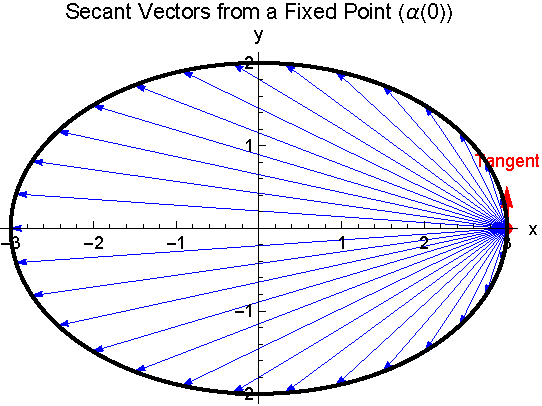
\includegraphics[width=0.4\textwidth,height=0.3\textwidth]{hopf_secants.pdf} % Adjust width as needed
    \caption{Illustration of secant vectors from a fixed point on a closed curve,
             visualizing the $\Delta\phi_{start}$ component in the proof of Hopf's Umlaufsatz.}
    \label{fig:hopf_secants} % Label for cross-referencing
\end{figure}

\begin{remark}
    The theorem can be viewed as a 1-dimensional version of Gauss-Bonnet Formula.
\end{remark}

\subsection{Isoperimetric Inequality}

\begin{theorem}[Isoperimetric Inequality]
    Let $\alpha$ be a simple closed plane curve. Let A be the area bounded by curves, then $L^2\geq 4\pi A$
\end{theorem}
\begin{proof}
The proof compares the area of the given curve $\mathcal{C}$ to that of a circle $\mathcal{S}^1$ by relating their parametrizations.

\paragraph{Step 1: The Setup.}
Let $\mathcal{C}$ be a simple closed curve of length $L$ enclosing area $A$. We can parameterize $\mathcal{C}$ by arc length, $\gamma(t) = (x(t), y(t))$ for $t \in [0, L]$. A key property of this parametrization is that the tangent vector has unit length:
\[ (x'(t))^2 + (y'(t))^2 = 1 \]
We construct a circle $\mathcal{S}^1$ of an arbitrary radius $r$ centered at the origin. We then define a new curve, $\beta(t) = (x(t), \tilde{y}(t))$, which traces this circle using the same x-coordinate as $\gamma(t)$. To ensure $\beta(t)$ remains on the circle, we must have $\tilde{y}(t) = \pm\sqrt{r^2 - x(t)^2}$.
% For the Isoperimetric Inequality illustration
\begin{figure}[h!]
    \centering
    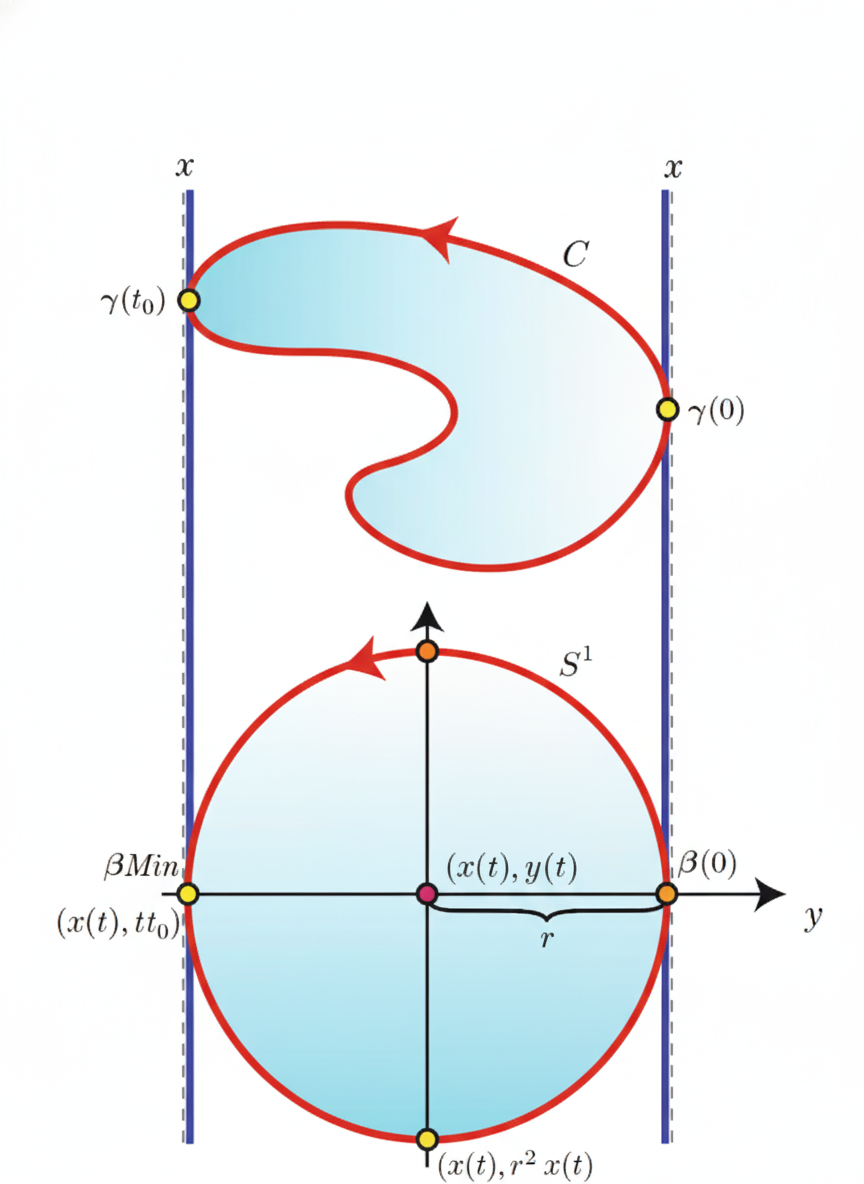
\includegraphics[width=0.5\textwidth]{isoperimetric_proof.png} % Adjust width
    \caption{Geometric construction for the proof of the Isoperimetric Inequality.
             Curve C (red) and constructed circle S\textsuperscript{1} (blue) sharing x-coordinates.}
    \label{fig:isoperimetric_proof}
\end{figure}

\paragraph{Step 2: Combining the Area Formulas.}
Using Green's Theorem, we can express the areas as line integrals:
\begin{itemize}
    \item The area of $\mathcal{C}$ is $A = \int_0^L x(t)y'(t) \, dt$.
    \item The area of the circle $\mathcal{S}^1$ is $\pi r^2 = -\int_0^L \tilde{y}(t)x'(t) \, dt$.
\end{itemize}
Adding these two expressions for area yields:
\[ A + \pi r^2 = \int_0^L \left( x(t)y'(t) - \tilde{y}(t)x'(t) \right) \, dt \]

\paragraph{Step 3: Applying the Cauchy-Schwarz Inequality.}
The integrand can be interpreted as the dot product of two vectors, $\mathbf{v}_1(t) = (x(t), -\tilde{y}(t))$ and $\mathbf{v}_2(t) = (y'(t), x'(t))$. We apply the Cauchy-Schwarz inequality for integrals, which states $\int \mathbf{v}_1 \cdot \mathbf{v}_2 \, dt \le \int ||\mathbf{v}_1|| \, ||\mathbf{v}_2|| \, dt$.
\[ A + \pi r^2 \le \int_0^L \sqrt{x(t)^2 + (-\tilde{y}(t))^2} \cdot \sqrt{y'(t)^2 + x'(t)^2} \, dt \]
The terms in the integral simplify significantly:
\begin{itemize}
    \item Since $\beta(t)$ is on the circle, $\sqrt{x(t)^2 + \tilde{y}(t)^2} = \sqrt{r^2} = r$.
    \item Since $\gamma(t)$ is parameterized by arc length, $\sqrt{y'(t)^2 + x'(t)^2} = 1$.
\end{itemize}
Substituting these back, the inequality becomes:
\[ A + \pi r^2 \le \int_0^L r \cdot 1 \, dt = rL \]

\paragraph{Step 4: Finding the Optimal Bound.}
We have derived the relation $A \le rL - \pi r^2$, which must hold for any choice of $r > 0$. To find the tightest possible bound for $A$, we find the value of $r$ that maximizes the function $f(r) = rL - \pi r^2$. Taking the derivative with respect to $r$ and setting it to zero gives:
\[ f'(r) = L - 2\pi r = 0 \implies r = \frac{L}{2\pi} \]
This is the radius of a circle with perimeter $L$. Substituting this optimal radius back into our inequality yields:
\begin{align*}
    A &\le \left(\frac{L}{2\pi}\right)L - \pi\left(\frac{L}{2\pi}\right)^2 \\
    A &\le \frac{L^2}{2\pi} - \pi\left(\frac{L^2}{4\pi^2}\right) \\
    A &\le \frac{L^2}{2\pi} - \frac{L^2}{4\pi} \\
    A &\le \frac{L^2}{4\pi}
\end{align*}
Rearranging this gives the isoperimetric inequality: $4\pi A \le L^2$.

\paragraph{The Equality Case.}
Equality holds if the Cauchy-Schwarz inequality becomes an equality, which occurs if and only if the vectors $\mathbf{v}_1(t)$ and $\mathbf{v}_2(t)$ are parallel for all $t$. This means $\mathbf{v}_1(t) = k \, \mathbf{v}_2(t)$ for some scalar $k$. The magnitudes must also be equal, so $|k| \cdot ||\mathbf{v}_2|| = ||\mathbf{v}_1||$, which gives $|k| \cdot 1 = r$, so $k = \pm r$.

This implies that $x(t) = \pm r y'(t)$ and $-\tilde{y}(t) = \pm r x'(t)$. For the parametrizations to match, the original curve $\gamma(t)$ must itself be a circle of radius $r$. Since the optimal radius was $r = L/(2\pi)$, equality holds if and only if $\mathcal{C}$ is a circle.
\end{proof}

\subsection{Four vertex Theorem (Covered in Tutorial)}

We begin by defining the key concepts required for the theorem and its proof. Let $\gamma(t) = (x(t), y(t))$ be a regular plane curve.

\begin{definition}[Signed Curvature]
For a regular plane curve $\gamma(t)$ parameterized by arc length $s$, its velocity vector is $\mathbf{v}(s) = \gamma'(s)$ and its acceleration is $\mathbf{a}(s) = \gamma''(s)$. The signed curvature, $k_s(s)$, is defined by the relation $\mathbf{a}(s) = k_s(s) R_{90}(\mathbf{v}(s))$, where $R_{90}$ is a 90-degree counter-clockwise rotation. For a general parameter $t$, the curvature equations are:
\begin{align}
    x''(t) &= -k_s(t)y'(t) \\
    y''(t) &= k_s(t)x'(t)
\end{align}
\end{definition}

\begin{definition}[Vertex]
A point $\gamma(t)$ on the trace of a regular plane curve is called a \textbf{vertex} if the signed curvature function $k_s$ has a local maximum or a local minimum at $t$.
\end{definition}

\begin{definition}[Convex Curve]
A simple closed plane curve is called \textbf{convex} if its trace lies entirely on one closed side of each of its tangent lines.
\end{definition}

Now we state the four vertex theorem.

\begin{theorem}[The Four Vertex Theorem]
\label{thm:four_vertex}
Every simple closed plane curve has at least four vertices.
\end{theorem}

\noindent
\textit{Note: The following proof addresses the special case where the curve is convex.}

The proof relies on the following geometric property of convex curves.

\begin{lemma}
\label{lem:convexity}
Let $C$ be the trace of a simple closed convex plane curve, and let $L$ be a line. If $L$ intersects $C$ in at least three points, then $C$ must contain the entire line segment of $L$ between any pair of these points.
\end{lemma}

\noindent
A direct consequence is that if a line is not part of the curve, it can intersect a convex curve at most twice.


\begin{proof}[Proof of Theorem \ref{thm:four_vertex} for Convex Curves]
The proof is by contradiction.

\paragraph{Step 1: The Contradiction Hypothesis.}
Assume there exists a simple, closed, convex curve $\gamma$ with fewer than four vertices. Since the continuous curvature function $k_s$ on a closed curve must attain a global maximum and a global minimum, the curve must have at least two vertices. As local maxima and minima must alternate, the number of vertices must be even. Therefore, our assumption implies that $\gamma$ has exactly two vertices:
\begin{itemize}
    \item A point $p$ where $k_s$ attains its global maximum.
    \item A point $q$ where $k_s$ attains its global minimum.
\end{itemize}

\paragraph{Step 2: Geometric Setup.}
Let $L$ be the line passing through the points $p$ and $q$. By Lemma \ref{lem:convexity}, since the curve is convex and not a line segment, $L$ can intersect the curve only at points $p$ and $q$.

We can apply a rigid motion (translation and rotation) to the curve to simplify our coordinate system without changing its geometric properties. We set up the coordinates such that:
\begin{itemize}
    \item The point $p$ is at the origin, $p=(0,0)$.
    \item The line $L$ is the x-axis.
    \item The point $q$ is on the positive x-axis, $q=(a,0)$ for some $a>0$.
\end{itemize}
Let the curve be parameterized by $\gamma(t) = (x(t), y(t))$ for $t \in [0, l]$.

\paragraph{Step 3: Analysis of the Functions.}
From our setup, the entire curve lies on one side of the x-axis. We can assume without loss of generality that $y(t) \ge 0$ for all $t \in [0,l]$.
Furthermore, for a positively oriented (counter-clockwise) simple closed convex curve, the signed curvature $k_s(t)$ is strictly positive.

Therefore, the product of these two functions, $y(t)k_s(t)$, must be non-negative for all $t$, and it is only zero at the points $p$ and $q$.

\paragraph{Step 4: The Contradiction.}
We analyze the integral of the product $y(t)k_s(t)$ over the entire curve.
\begin{enumerate}
    \item \textbf{The integral must be positive.} Since $y(t)k_s(t) \ge 0$ for all $t$ and is not identically zero, its integral must be strictly positive:
    $$ \int_0^l y(t)k_s(t) \, dt > 0 $$

    \item \textbf{The integral must be zero.} However, as stated in the textbook's argument, integrating by parts and using the curvature equations from (1) and (2) shows that the integral is zero. A key part of such a derivation involves using the fact that for a closed curve, the integral of an exact derivative is zero. For example, using equation (2), $y''(t) = k_s(t)x'(t)$, we know:
    $$ \int_0^l k_s(t)x'(t) \, dt = \int_0^l y''(t) \, dt = \left[ y'(t) \right]_0^l = 0 $$
    The textbook asserts that a similar line of reasoning (though not fully detailed) leads to the conclusion that our original integral is zero.
\end{enumerate}

We have reached a contradiction: the integral cannot be both strictly positive and equal to zero. Thus, our initial assumption that the curve has fewer than four vertices must be false. This completes the proof.
\end{proof}
\newpage
\section{Local Theory of Surfaces}
\subsection{Introduction}
\begin{definition}
A \textbf{parameterized surface} is a function $X: U \subseteq \mathbb{R}^2 \rightarrow \mathbb{R}^3$ where $Z$ is differentiable. We say $Z$ is \textbf{regular} if the Jacobian matrix
\[
dX= \begin{pmatrix}
\frac{\partial x}{\partial u} & \frac{\partial x}{\partial v} \\
\frac{\partial y}{\partial u} &\frac{\partial y}{\partial v} \\
\frac{\partial z}{\partial u} &\frac{\partial z}{\partial v}
\end{pmatrix}
\]
has rank 2 for all points in $U$. In coordinates:
\[
X(u,v) = (x(u,v), y(u,v), z(u,v))
\]
Equivalently, $Z: U \subseteq \mathbb{R}^2 \rightarrow \mathbb{R}^3$ is an embedding. The image $Z(U)$ is called the \textbf{trace} of $Z$.
\end{definition}

\begin{remark}
For regular curves $\alpha: I \rightarrow \mathbb{R}^3$, we require $\alpha' \neq 0$. For surfaces, the analogous condition is that the differential has full rank.
\end{remark}

\begin{example}
    Consider the parameterization:
\[
X: (0,2\pi) \times (0,\pi) \rightarrow \mathbb{R}^3
\]
\[
X(\theta, \varphi) = (r\cos\theta\sin\varphi, r\sin\theta\sin\varphi, r\cos\varphi)
\]


This parameterization $Z$ is regular because
\[
\frac{\partial X}{\partial \theta} \times \frac{\partial X}{\partial \varphi} \neq 0
\]
and the Jacobian matrix has rank 2.

\end{example}
As in the case of curves. We wish to parametrize a surface to do Calculus on surfaces. Of course we need two variables rather than 1 variable in the curve case.
\begin{remark}[Problem of the parametrized surface]
The above example of ${S}^2$ reveals that in order to develop a unified theory for studying surfaces, it is necessary to use more than one coordinate patch. Now we would like to introduce the concept of regular surface.  
\end{remark}
\begin{definition}
A subset $S \subset \mathbb{R}^3$ is a \textbf{regular surface} if for every point $p \in S$, there exists a neighborhood $V \subset \mathbb{R}^3$ of $p$ (which can be taken as an open ball centered at $p$ with radius $r > 0$) and a map $X: U \rightarrow V \cap S$ where $U \subset \mathbb{R}^2$ is open and connected, such that:

\begin{enumerate}
    \item $X$ is differentiable: 
    \[
    X(u,v) = (x(u,v), y(u,v), z(u,v)), \quad (u,v) \in U
    \]
    has partial derivatives of all orders.
    
    \item $X$ is bijective with continuous inverse $X^{-1}$, i.e., $X$ is a homeomorphism.
    
    \item (Regularity) For $q \in U$ with $X(q) = p$, the Jacobian matrix
    \[
    dX_q = \begin{pmatrix}
    \frac{\partial x}{\partial u} & \frac{\partial x}{\partial v} \\
    \frac{\partial y}{\partial u} & \frac{\partial y}{\partial v} \\
    \frac{\partial z}{\partial u} & \frac{\partial z}{\partial v}
    \end{pmatrix}
    \]
    has rank 2 for all $q \in U$.
\end{enumerate}
\end{definition}

\begin{remark}
    Conditions (2) and (3) together guarantee that $X$ is an embedding from $U$ to $S$, ensuring the existence of a tangent plane at each point of $S$. This is analogous to the requirement $\alpha' \neq 0$ for regular curves.
\end{remark}

\begin{example}
Let $S^2 = \{(x,y,z) \in \mathbb{R}^3 \mid x^2 + y^2 + z^2 = 1\}$ be the unit sphere. We can cover $S^2$ using 6 coordinate patches. For example, let
\[
U = \{(x,y) \in \mathbb{R}^2 \mid x^2 + y^2 < 1\}
\]
and define the coordinate patch for the upper hemisphere:
\[
X(x,y) = \left(x, y, \sqrt{1 - x^2 - y^2}\right), \quad (x,y) \in U
\]
And then we can do the same for other coordinates.
\end{example}

\begin{example}
    Suppose $f: U \subseteq \mathbb{R}^2 \rightarrow \mathbb{R}$ is a smooth map. Then the graph of $f$ defined as
\[
S = \operatorname{graph}(f) = \{(x, y, z) \in \mathbb{R}^3 \mid (x, y) \in U, z = f(x, y)\}
\]
is a regular surface.\newline
\noindent \underline{Homework}: Check the graph is indeed a regular surface.
\end{example}

The above example shows that graph is a regular surface, and indeed the converse is in some sense true. Every regular surface is Locally a graph.

\begin{proposition}
Any regular surface $S$ is locally a graph.
\end{proposition}

\begin{proof}
Let $p \in S$ be any point and let $X: U \rightarrow V \cap S$ be the coordinate patch given in the definition of regular surfaces, with $X(q) = p$. By the regularity condition, the differential
\[
dX_q = \begin{pmatrix}
\frac{\partial X}{\partial u} & \frac{\partial X}{\partial v}
\end{pmatrix}
\]
has rank 2. This means that among the three possible $2 \times 2$ Jacobian matrices:
\[
\begin{pmatrix}
\frac{\partial x}{\partial u} & \frac{\partial x}{\partial v} \\
\frac{\partial y}{\partial u} & \frac{\partial y}{\partial v}
\end{pmatrix}, \quad
\begin{pmatrix}
\frac{\partial x}{\partial u} & \frac{\partial x}{\partial v} \\
\frac{\partial z}{\partial u} & \frac{\partial z}{\partial v}
\end{pmatrix}, \quad
\begin{pmatrix}
\frac{\partial y}{\partial u} & \frac{\partial y}{\partial v} \\
\frac{\partial z}{\partial u} & \frac{\partial z}{\partial v}
\end{pmatrix}
\]
at least one has nonzero determinant.

Without loss of generality, assume the first Jacobian matrix has nonzero determinant. Then by the inverse function theorem, the projection
\[
\pi \circ X: (u,v) \mapsto (x(u,v), y(u,v))
\]
has a differentiable inverse in some neighborhood of $q$.

Let $g = (\pi \circ X)^{-1}$ be this inverse mapping, which sends $(x,y) \mapsto (u(x,y), v(x,y))$. Then we have
\[(x,y)\to (u,v)\to (x,y,z(x(u,v),y(u,v)))\]
By the formulas we see that indeed it is locally a graph.
\end{proof}
\begin{remark}
    The above proof is a routine technique to apply the inverse function/implicit function theorem in geometry.
\end{remark}

\begin{example}
Let $f: \mathbb{R}^3 \rightarrow \mathbb{R}$ be a smooth map and $a \in \mathbb{R}$ be such that for all $p \in f^{-1}(a)$, the differential $(df)_p \neq 0$ (i.e., $a$ is a regular value of $f$). Then $f^{-1}(a) \subset \mathbb{R}^3$ is a regular surface.
\begin{proof}
For any $p \in f^{-1}(a)$, suppose without loss of generality that $\left(\frac{\partial f}{\partial z}\right)_p \neq 0$.

Define the function $F: \mathbb{R}^3 \rightarrow \mathbb{R}$ by:
\[
F(x) = f(x) - a
\]
Then $F(p) = 0$.

Since $\left(\frac{\partial F}{\partial z}\right)_p = \left(\frac{\partial f}{\partial z}\right)_p \neq 0$, by the implicit function theorem, there exists a smooth function $g: U \subset \mathbb{R}^2 \rightarrow \mathbb{R}$ such that:
\[
F(u, g(u)) = 0 \quad \forall u \in U
\]
where $U$ is an open neighborhood in $\mathbb{R}^2$.

This means we can express a neighborhood of $p \in f^{-1}(a)$ as:
\[
W = \{(u, g(u)) \mid u \in U\}, \quad \text{with } p = (u_0, g(u_0))
\]

Therefore, there exists a neighborhood $V$ such that:
\[
V \cap f^{-1}(a) = \{(x, y, z) \mid (x, y) \in U, z = g(x, y)\}
\]

This shows that every point $p \in f^{-1}(a)$ is locally a graph, hence by the previous proposition about graphs of functions being regular surfaces, $f^{-1}(a)$ is a regular surface.
\end{proof}
\end{example}

\begin{example}
Consider the ellipsoid defined by the equation:
\[
\frac{x^2}{a^2} + \frac{y^2}{b^2} + \frac{z^2}{c^2} = 1
\]
where $a, b, c > 0$ are constants.
\begin{proof}
Define the function $F: \mathbb{R}^3 \rightarrow \mathbb{R}$ by:
\[
F(x, y, z) = \frac{x^2}{a^2} + \frac{y^2}{b^2} + \frac{z^2}{c^2} - 1
\]

Then:
\begin{enumerate}
    \item $F$ is obviously differentiable (in fact, smooth) on $\mathbb{R}^3$
    
    \item The differential of $F$ is given by:
    \[
    dF = \left( \frac{\partial F}{\partial x}, \frac{\partial F}{\partial y}, \frac{\partial F}{\partial z} \right) = \left( \frac{2x}{a^2}, \frac{2y}{b^2}, \frac{2z}{c^2} \right)
    \]
    
    \item For any point $w = (w_1, w_2, w_3) \in F^{-1}(0)$ (i.e., on the ellipsoid), we have:
    \[
    dF(w) = \left( \frac{2w_1}{a^2}, \frac{2w_2}{b^2}, \frac{2w_3}{c^2} \right)
    \]
    
    Since $w$ lies on the ellipsoid, at least one coordinate must be nonzero, hence $dF(w) \neq 0$. Therefore, 0 is a regular value of $F$.
\end{enumerate}

By the regular value theorem, $F^{-1}(0)$ is a regular surface.
\end{proof}
\end{example}

\begin{remark}
    For the sphere $S^2$,it is possible to cover the surface using only 2 coordinate patches. See Streographic Peojection.
\end{remark}
\begin{example}[Stereographic Projection]
    See Homework.
\end{example}
\subsection{Change of Coordinates}
Recall that for curves, we may have different parametrizations. The same holds for regular surfaces. We say that two parametrizations describe the same surface even if they use different coordinate systems.

\begin{proposition}
Let $p \in S$ be a point in the image of two parametrizations:
\[
X: U \rightarrow S \quad \text{and} \quad Y: V \rightarrow S
\]
Let $W = X(U) \cap Y(V)$ be the overlapping region. Then the transition map
\[
\varphi = X^{-1} \circ Y: Y^{-1}(W) \rightarrow X^{-1}(W)
\]
defined by $(u,v) \mapsto (u',v')$ is a diffeomorphism.
\end{proposition}

\begin{proof}
Since both $X$ and $Y$ are regular parametrizations, they are homeomorphisms onto their images and their differentials have full rank. Therefore:

1. $\varphi$ is well-defined as a map between open subsets of $\mathbb{R}^2$

2. $\varphi$ is a homeomorphism because it is the composition of homeomorphisms

3. $\varphi$ is differentiable because both $X$ and $Y$ are differentiable and regular

4. The inverse $\varphi^{-1} = Y^{-1} \circ X$ is similarly differentiable

The Jacobian matrix of the transition map is given by:
\[
d\varphi = \begin{pmatrix}
\frac{\partial u'}{\partial u} & \frac{\partial u'}{\partial v} \\
\frac{\partial v'}{\partial u} & \frac{\partial v'}{\partial v}
\end{pmatrix}
\]
This matrix is invertible everywhere because $\varphi$ is a diffeomorphism.
\end{proof}
\begin{remark}
This property is fundamental in manifold theory. It ensures that geometric properties defined using different coordinate systems are consistent. The transition maps allow us to define a smooth structure on the surface $S$ by specifying how different coordinate patches relate to each other.
This is exactly the property we aim to generalize in the theory of smooth manifolds, where we use charts and transition maps to define the smooth structure.
\end{remark}

\subsection{Tangent plane}
\begin{definition}
Let $\mathbf{x}: U \to \text{VAS}$ be a coordinate patch of a regular surface at a $\text{pt } \mathbf{x}(p) = p \in S$. Then the tangent plane at $p \in S$ is defined as
\[
T_p S = \text{Im} \left( (\mathrm{d}\mathbf{x})_p \right) = \text{span} \left\{ \frac{\partial \mathbf{x}}{\partial u} (p), \frac{\partial \mathbf{x}}{\partial v} (p) \right\}.
\]
\end{definition}

\begin{definition}
The normal vector of a $\text{pt } p$ on a coordinate patch $\mathbf{x}: U \to \text{VAS}$ is defined as
\[
N(p) = \frac{\frac{\partial \mathbf{x}}{\partial u} \times \frac{\partial \mathbf{x}}{\partial v}}{\left\| \frac{\partial \mathbf{x}}{\partial u} \times \frac{\partial \mathbf{x}}{\partial v} \right\|} \quad (p)
\]
\end{definition}

\noindent \underline{Problem:} 
although the tangent plane is well-defined, but $N(p)$ may be affected by our choice of coordinates. (the sign).

\begin{definition}
A tangent vector at $p \in S$ is the tangent vector $\alpha'(0)$ of a regular curve $\alpha: (-\varepsilon, \varepsilon) \to S \subseteq \mathbb{R}^3$ with $\alpha(0) = p$.
\end{definition}

\begin{proposition}
The set of tangent vectors at $p \in S$ is precisely equal to $T_p S$.
\end{proposition}

\begin{proof}
Let $\alpha: (-\varepsilon, \varepsilon) \to S$ be regular with $\alpha(0)=p$.
Recall that $\exists \ V$ of $p \in S$ such that by restricting $\text{VAS}$ to $V \cap S$, we have $\mathbf{y}: U' \to V \cap S$
such that $\mathbf{y}(u', v') = (u', v', f(u', v'))$
or $(u', g(u', v'), v')$ (locally a graph).

we look at the first case. w.l.o.g. by making $\varepsilon$ small enough.
assume $\alpha(-\varepsilon, \varepsilon) \subseteq V \cap S$.

Let $\beta$ be given by $\beta: (-\varepsilon, \varepsilon) \to U' \subseteq \mathbb{R}^2$
where $\mathbf{y}^{-1}$ is differentiable. ($\mathbf{y}^{-1}$ is just the projection map)
Then $\alpha = \mathbf{y} \circ \beta = \mathbf{x} \circ (\mathbf{x}^{-1} \circ \mathbf{y} \circ \beta)$

we've seen in prop that $\mathbf{x}^{-1} \circ \mathbf{y}$ is differentiable
so $\alpha'(0) = (\mathrm{d}\mathbf{x})_q \cdot (\mathrm{d}(\mathbf{x}^{-1} \circ \mathbf{y} \circ \beta)) (0)$
\[
= \left( \frac{\partial \mathbf{x}}{\partial u}, \frac{\partial \mathbf{x}}{\partial v} \right)_q \begin{pmatrix} a \\ b \end{pmatrix}
\]
$\Rightarrow \alpha'(0) \in T_p S$.
We've just seen that $\alpha'(0) \in T_p S$.

Now we must to see $\mathbf{w} \in T_p S \Rightarrow \mathbf{w} = \alpha'(0)$ for some $\alpha$.
Suppose $\mathbf{w} = \left( \frac{\partial \mathbf{x}}{\partial u} (p), \frac{\partial \mathbf{x}}{\partial v} (p) \right) \begin{pmatrix} a \\ b \end{pmatrix} \in T_p S$.
Then let $\beta: (-\varepsilon, \varepsilon) \to U$ by $\beta(t) = p + t \begin{pmatrix} a \\ b \end{pmatrix}$.
and $\alpha = \mathbf{x} \circ \beta$. Then $\alpha(0) = \mathbf{x}(\beta(0)) = \mathbf{x}(p) = p$.
$\alpha'(0) = (\mathrm{d}\mathbf{x})_p \cdot \mathrm{d}\beta_0 = \left( \frac{\partial \mathbf{x}}{\partial u}, \frac{\partial \mathbf{x}}{\partial v} \right) \begin{pmatrix} a \\ b \end{pmatrix} \in T_p S$.
\end{proof}
\begin{example}
    Suppose $f: \mathbb{R}^3 \to \mathbb{R}$ smooth. $S = f^{-1}(a)$.
Let $\alpha: (-\varepsilon, \varepsilon) \to S$ with $\alpha(0)=p$. Then
\[
f(\alpha(t)) = f(x(t), y(t), z(t)) = a.
\]
Differentiating with respect to $t$:
\[
\Rightarrow (\mathrm{d}f)_p \cdot (\mathrm{d}\alpha)_0 = 0.
\]
\[
\Rightarrow (\mathrm{d}f)_p \cdot \alpha'(0) = 0.
\]
$\Rightarrow (\mathrm{d}f)_p$ is always normal to $T_p S$.
\end{example}

\noindent \underline{Question:} we define $N(p)$ on a coordinate patch. can we choose coordinates patch appropriately so that $N: S \to \mathbb{R}^3$ is a smooth function?

\begin{remark}
    When we move from local to global, it is always determined by the "topology" property.
\end{remark}

\subsection{First Fundamental Form }
After defining the tangent plane, we wil study the inner product structure so that we can compute the area of the surface.

\begin{definition}
    Let $V$ be a vector space. We study $\langle \cdot, \cdot \rangle : V \times V \to \mathbb{R}$ an inner product if it satisfies the following:
\begin{enumerate}
    \item $\langle \mathbf{v}, \mathbf{w} \rangle = \langle \mathbf{w}, \mathbf{v} \rangle$ (symmetric).
    \item $\langle a\mathbf{v}_1 + b\mathbf{v}_2, \mathbf{w} \rangle = a \langle \mathbf{v}_1, \mathbf{w} \rangle + b \langle \mathbf{v}_2, \mathbf{w} \rangle$ (linearity).
    \item $\langle \mathbf{v}, \mathbf{v} \rangle \ge 0 \quad \forall \mathbf{v} \in V$. equality holds if and only if $\mathbf{v}=\mathbf{0}$.
\end{enumerate}
\end{definition}

\begin{definition}
The quadratic form corresponding to an inner product is a map $q: V \to \mathbb{R}$ defined by
\[
\mathbf{v} \to \langle \mathbf{v}, \mathbf{v} \rangle.
\]
\end{definition}

\begin{definition}
The \textbf{First Fundamental Form} of $S$ is given by the quadratic form $I_p(\mathbf{v}) = \langle \mathbf{v}, \mathbf{v} \rangle$ for $\mathbf{v} \in T_p S$.
\end{definition}
In order to understand $I_p$ better, we need to choose a basis of $T_p S$ and express $I_p$ using matrices and vectors.

Let $\mathbf{x}: U \to \text{VAS}$ be a coordinate patch with $\mathbf{x}(p)=p$.
Then $\mathcal{B} = \left\{ \mathbf{x}_u = \frac{\partial \mathbf{x}}{\partial u} (p), \mathbf{x}_v = \frac{\partial \mathbf{x}}{\partial v} (p) \right\}$
\begin{align*}
\text{with } E_p &= \langle \mathbf{x}_u, \mathbf{x}_u \rangle_p \\
F_p &= \langle \mathbf{x}_u, \mathbf{x}_v \rangle_p \\
G_p &= \langle \mathbf{x}_v, \mathbf{x}_v \rangle_p
\end{align*}
(We drop the subscript $p$ if it does not cause confusion)

Then for all $\mathbf{v}$, $I_p(\mathbf{v}) = (a, b) \begin{pmatrix} E & F \\ F & G \end{pmatrix} \begin{pmatrix} a \\ b \end{pmatrix}$.

More precisely, $\langle \mathbf{v}, \mathbf{w} \rangle_p = (a, b) \begin{pmatrix} E & F \\ F & G \end{pmatrix} \begin{pmatrix} c \\ d \end{pmatrix}$, where $\mathbf{v} = a \mathbf{x}_u + b \mathbf{x}_v$ and $\mathbf{w} = c \mathbf{x}_u + d \mathbf{x}_v$.

Therefore, in a coordinate patch $\text{IFF}$ refers to $\begin{pmatrix} E & F \\ F & G \end{pmatrix}$.

\begin{example}
\begin{enumerate}
    \item \textbf{Cylinder:}
    \[
    \mathbf{x}(u, v) = (\cos u, \sin u, v)
    \]
    \[
    \mathbf{x}_u = (-\sin u, \cos u, 0)
    \]
    \[
    \mathbf{x}_v = (0, 0, 1)
    \]
    $E = \langle \mathbf{x}_u, \mathbf{x}_u \rangle = 1. \quad F = 0. \quad G = 1.$
    \[
    \Rightarrow I_p = \begin{pmatrix} E & F \\ F & G \end{pmatrix} = \begin{pmatrix} 1 & 0 \\ 0 & 1 \end{pmatrix}
    \]

    \item \textbf{Plane:}
    \[
    \mathbf{x}(u, v) = \mathbf{x}_0 + u \mathbf{w}_1 + v \mathbf{w}_2
    \]
    (Assuming $\mathbf{w}_1$ and $\mathbf{w}_2$ are orthonormal, $\langle \mathbf{w}_i, \mathbf{w}_j \rangle = \delta_{ij}$)
    \[
    I_p = \begin{pmatrix} 1 & 0 \\ 0 & 1 \end{pmatrix}
    \]

    \item
    \[
    \mathbf{x}(u, v) = (u, v, \sqrt{1-u^2-v^2})
    \]
    \[
    \mathbf{x}_u = \left( 1, 0, \frac{-u}{\sqrt{1-u^2-v^2}} \right), \quad \mathbf{x}_v = \left( 0, 1, \frac{-v}{\sqrt{1-u^2-v^2}} \right)
    \]
    \[
    I_p = \begin{pmatrix}
        \frac{1-v^2}{1-u^2-v^2} & \frac{uv}{1-u^2-v^2} \\
        \frac{uv}{1-u^2-v^2} & \frac{1-u^2}{1-u^2-v^2}
    \end{pmatrix}
    \]
    (Note: This is the IFF for the upper hemisphere in Cartesian coordinates.)
    $\mathbf{\tilde{x}}_\varphi = (-\sin \phi \sin \varphi, \sin \phi \cos \varphi, 0)$.
% IFF for the sphere in spherical coordinates, assuming u=\phi, v=\varphi
\[
I_p = \begin{pmatrix} 1 & 0 \\ 0 & \sin^2 \phi \end{pmatrix} \quad \text{different expression of } I_p \text{ for the same surface } S
\]
\end{enumerate}
\end{example}

\noindent \underline{Question:}
Suppose we have 2 parameterizations
\[
\mathbf{x}: U \to V \cap S, \quad \mathbf{\tilde{x}}: \tilde{U} \to V \cap S.
\]
Note that
\[
\begin{pmatrix} \tilde{E} & \tilde{F} \\ \tilde{F} & \tilde{G} \end{pmatrix} = \left( \frac{\partial \mathbf{\tilde{x}}}{\partial \tilde{u}}, \frac{\partial \mathbf{\tilde{x}}}{\partial \tilde{v}} \right)^T \begin{pmatrix} \frac{\partial \mathbf{\tilde{x}}}{\partial \tilde{u}} \\ \frac{\partial \mathbf{\tilde{x}}}{\partial \tilde{v}} \end{pmatrix}
= (\mathrm{d}\mathbf{\tilde{x}})^T \mathrm{d}\mathbf{\tilde{x}}.
\]
Suppose $\Psi = \mathbf{x}^{-1} \circ \mathbf{\tilde{x}}$ is the transition function
\[
\Psi(\tilde{u}, \tilde{v}) = (u(\tilde{u}, \tilde{v}), v(\tilde{u}, \tilde{v})).
\]
\[
\Rightarrow \mathbf{\tilde{x}} = \mathbf{x} \circ \Psi. \quad \text{so}
\]
\[
\mathrm{d}\mathbf{\tilde{x}} = \mathrm{d}\mathbf{x} \mathrm{d}\Psi, \quad \text{and hence}
\]
\begin{align*}
\begin{pmatrix} \tilde{E} & \tilde{F} \\ \tilde{F} & \tilde{G} \end{pmatrix} &= (\mathrm{d}\mathbf{x} \mathrm{d}\Psi)^T (\mathrm{d}\mathbf{x} \mathrm{d}\Psi) \\
&= (\mathrm{d}\Psi)^T (\mathrm{d}\mathbf{x})^T (\mathrm{d}\mathbf{x}) (\mathrm{d}\Psi) \\
&= (\mathrm{d}\Psi)^T \begin{pmatrix} E & F \\ F & G \end{pmatrix} (\mathrm{d}\Psi)
\end{align*}
composition by \textbf{Jacobian matrix}.

\begin{example} Back to the sphere example.
\[
\Psi(\phi, \varphi) = (\sin \phi \cos \varphi, \sin \phi \sin \varphi)
\]
$\mathrm{d}\Psi = \begin{pmatrix}
\cos\phi \cos\varphi & -\sin\phi \sin\varphi \\
\cos\phi \sin\varphi & \sin\phi \cos\varphi
\end{pmatrix}$
and
\[
(\mathrm{d}\Psi)^T \begin{pmatrix} E & F \\ F & G \end{pmatrix} \mathrm{d}\Psi = \begin{pmatrix} 1 & \mathbf{0} \\ \mathbf{0} & \sin^2 \phi \end{pmatrix}
\]
\end{example}

\begin{corollary}
\[
\sqrt{\tilde{E}\tilde{G}-\tilde{F}^2} = \sqrt{EG-F^2} \ \det \left( \frac{\partial (u, v)}{\partial (\tilde{u}, \tilde{v})} \right)
\]
\begin{remark}
    We are always working in the orientable cases.
\end{remark}
\end{corollary}

With the first fundamental form, we can compute arc-length, area, etc.

\begin{enumerate}
    \item Arc-length.
    $$L(\gamma) = \int_I |\gamma'(t)| \, dt$$
    $$\gamma'(t) = X_u(u, v) u'(t) + X_v(u, v) v'(t)$$
    $$= \int_I \sqrt{|X_u u'(t) + X_v v'(t)|^2} \, dt$$
    $$= \int_I \sqrt{E |u'(t)|^2 + 2F u'(t) v'(t) + G |v'(t)|^2} \, dt.$$
    (If we consider $\gamma$ a curve on $S$ then first fundamental form gives us \textbf{Advantage}: a way to determine the arc-length \textbf{intrinsically}.)

    We just need to know $\alpha(t) = (x(t), y(t))$ to compute the arc-length of $\alpha$.

    \item Area of Surface
    \begin{definition}
        Let $Z: U \to S \cap V$ be a coordinate patch of $S$, and $R \in S$ be such that $Z(U) = R$ for $U \subset \mathbb{R}^2$. Then the area of $R$ is given by
        $$\int_A |X_u \times X_v| \, du \, dv.$$
    \end{definition}
    Note that $|u \times w|^2 = |u|^2 |w|^2 - (u \cdot w)^2$.
    That is $|X_u \times X_v| = \sqrt{EG - F^2}$.

    What happens if we have $\tilde{Z}: \tilde{U} \to S \cap \tilde{V}$ and $Z(U) = \tilde{Z}(\tilde{U}) = R$?
    Note that
    $$\Psi = Z^{-1} \circ \tilde{Z}: \tilde{U} \to U$$
    $$\int_{\tilde{R}} \sqrt{\tilde{E} \tilde{G} - \tilde{F}^2} \, d\tilde{u} \, d\tilde{v} = \int_R \sqrt{E G - F^2} \left|\frac{\partial(u, v)}{\partial(\tilde{u}, \tilde{v})}\right| \, d\tilde{u} \, d\tilde{v}$$
\end{enumerate}

$$= \int_R \sqrt{EG - F^2} \, du \, dv.$$
$$ \implies \text{Area of } R \text{ is independent of the choice of coordinate patch.}$$

\begin{remark}
    \textbf{Recall}:
    \begin{itemize}
        \item First fundamental form ($\text{f.f.f}$): $I_p(w) = \langle w, w \rangle, w \in T_p S$.
        \item If $X: U \to V \cap S$, $w = a X_u + b X_v$, then $I_p(w) = (a \ b) \begin{pmatrix} E & F \\ F & G \end{pmatrix} \begin{pmatrix} a \\ b \end{pmatrix}$.
    \end{itemize}
\end{remark}

\section{Gauss Map and the Second Fundamental Form}

\textbf{Main Goal}: Define curvature of a surface.

Recall that in the case of curves:
$$\vec{T}'(t) = \kappa(t) \vec{N}(t) \quad \text{in the case of plane curve.}$$
$$\vec{N}'(t) = -\kappa(t) \vec{T}(t)$$

So curvature of a plane curve can be measured by the changes of tangent/normal vector.

If we want to do this on surface, one would like to study the change of normal vector.

\textbf{Difficulty 1:}\\
The normal vector $N_p = \frac{X_u \times X_v}{\|X_u \times X_v\|}(q)$ is defined only up to a sign.

On each parametrization, one has a "smooth" choice of $N(p)$.
So we have:
$$N: V \cap S \to S^2$$
$$p \mapsto N(p) = \frac{X_u \times X_v}{\|X_u \times X_v\|}(q)$$

\begin{remark}
    \textbf{However}
    The map may not be able to be extended to whole $S$.
    For example, we have a problem defining $N: S \to S^2$ on a M\"obius band.
    The problem is the \textbf{orientability of $S$}.
\end{remark}

\begin{definition}
    Let $f: S_1 \to S_2$ be a map between two regular surfaces.
    We say $f$ is \textbf{smooth} if $Z_2^{-1} \circ f \circ Z_1$ is smooth.
    The surface $S$ is \textbf{orientable} if there is a smooth map
    $$N: S \to S^2$$
    such that $N(p) \perp T_p S$ for all $p \in S$.
\end{definition}

\begin{example}
    \begin{enumerate}
        \item Suppose $S$ is covered by one coordinate patch $Z: U \to S$.
        For example, $(S \text{ is the graph of a function } f)$.
        Then $N_{(p)} = \frac{X_u \times X_v}{\|X_u \times X_v\|}(q)$.
        \item Suppose $S = f^{-1}(0)$ is defined by an equation, then we can take
        $$N_{(p)} = \frac{D f(p)}{\|D f(p)\|} = \frac{(\frac{\partial f}{\partial x}, \frac{\partial f}{\partial y}, \frac{\partial f}{\partial z})}{|(\frac{\partial f}{\partial x}, \frac{\partial f}{\partial y}, \frac{\partial f}{\partial z})|} (p)$$
    \end{enumerate}
\end{example}

\textbf{Difficulty 2:} \\
For curves, we have $n' = -\kappa t$. For surfaces, we have two degrees of freedom on $S$.
\subsection{Gauss Map}
\begin{definition}
    The map $N$ is called \textbf{Gauss Map} of $S$. $N$ is well-defined up to a sign.
\end{definition}

\begin{definition}
    (Differential)
    Let $f: S_1 \to S_2$ be a map. The \textbf{differential} of $f$ at $p$, $d f_p$, is a map from $T_p S_1$ to $T_{f(p)} S_2$, defined by
    $$d f_p (v) := (f \circ \alpha)'(0),$$
    where $\alpha: (-\varepsilon, \varepsilon) \to S_1$ such that $\alpha(0) = p$, $\alpha'(0) = v$.
\end{definition}

\begin{remark}
    One needs to check this definition is well-defined.
    \textbf{Hint}: Instead of using the definition that $f$ is smooth if $\psi \circ f \circ \varphi^{-1}$ is smooth, one may use the definition that $f$ is smooth on $S_1 \subset \mathbb{R}^3$, if $f = F|_{S_1}$, where $F: \mathbb{R}^3 \to \mathbb{R}^3$ is smooth. It's much easier and intuitive in our cases.
\end{remark}

Now we study $d N_p: T_p S_1 \to T_{N(p)} S^2 \simeq T_p S$.
Geometrically, $d N_p$ measures how $N(p)$ changes along any direction of $T_p S$.

\begin{remark}
    One way to compute $d N_p: T_p S \to T_{N(p)} S^2$ is the following. Let $Z(u, v)$ coordinate patch of $S$.

    \begin{center}
        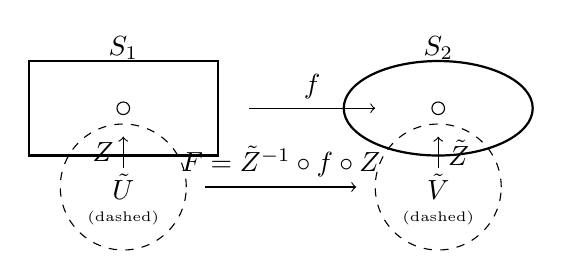
\begin{tikzpicture}[scale=0.8]
        \draw[thick] (0, 0) -- (3, 0) -- (3, 1.5) -- (0, 1.5) -- cycle;
        \node at (1.5, 1.7) {$S_1$};
        \draw (1.5, 0.75) circle (0.1);

        \draw[->] (3.5, 0.75) -- node[above] {$f$} (5.5, 0.75);

        \draw[thick] (6.5, 0.75) ellipse (1.5cm and 0.75cm);
        \node at (6.5, 1.7) {$S_2$};
        \draw (6.5, 0.75) circle (0.1);

        \node at (1.5, -0.5) {$\tilde{U}$};
        \node at (1.5, -1.0) {\tiny (dashed)};
        \draw[dashed] (1.5, -0.5) circle (1.0);
        \draw[->] (1.5, -0.2) -- node[left] {$Z$} (1.5, 0.3);

        \node at (6.5, -0.5) {$\tilde{V}$};
        \node at (6.5, -1.0) {\tiny (dashed)};
        \draw[dashed] (6.5, -0.5) circle (1.0);
        \draw[->] (6.5, -0.2) -- node[right] {$\tilde{Z}$} (6.5, 0.3);

        \draw[->] (2.8, -0.5) -- node[above] {$F = \tilde{Z}^{-1} \circ f \circ Z$} (5.2, -0.5);

        \end{tikzpicture}
    \end{center}

    If $w = a X_u + b X_v$,
    $$\begin{pmatrix} c \\ d \end{pmatrix} = \begin{pmatrix} \frac{\partial F_1}{\partial u} & \frac{\partial F_1}{\partial v} \\ \frac{\partial F_2}{\partial u} & \frac{\partial F_2}{\partial v} \end{pmatrix} \begin{pmatrix} a \\ b \end{pmatrix}$$
    $$(d f_p)(w) = c \tilde{Z}_{\tilde{u}} + d \tilde{Z}_{\tilde{v}}$$

    Consider $N \circ Z: U \to S^2$, by abuse of notation.
    Write this map as $N(u, v)$. ($\text{No } Z \text{ in that}$).

    To compute $d N_p$, take the "principal curve".
    $\beta(t) = (t, v_0)$. $\alpha = Z \circ \beta$. Has $\alpha'(0)=X_u$.
    Then $d N_p (X_u)$ is given by
    $$(N \circ \alpha)'(0) = (N \circ Z \circ \beta)'(0)$$
    $$= \frac{d}{d t} N(t, v_0)|_{t=0} = \frac{\partial N}{\partial u} = N_u.$$

    Similarly, $d N_p (X_v) = N_v = \frac{\partial N}{\partial v}$.

    Since $d N_p: T_p S \to T_{N(p)} S^2$ is a linear transformation
\end{remark}
% Uncertainty: The diagram illustrates $f: S_1 \to S_2$ and $F$ being the map between the parameter domains $\tilde{U}$ and $\tilde{V}$. However, the text immediately following the diagram relates to the differential $d f_p$, while the rest of the text focuses on the Gauss Map $N$. The first part of the remark seems to set up the general differential of a map $f$ (which is $d f_p$), while the second part is calculating $d N_p$ specifically. I've transcribed the content faithfully, including the diagram setup for the general differential.

And $\{X_u, X_v\}$ forms a basis of $T_p S$, one can get from
$$\begin{cases} d N_p (X_u) = N_u \\ d N_p (X_v) = N_v \end{cases}$$
Moreover, $\langle N, N \rangle = 1$, so differentiating yields $\langle d N, N \rangle = 0$.
$$\implies \langle N_u, N \rangle = 0 \implies N_u \in T_p S.$$
$$\implies \langle N_v, N \rangle = 0 \implies N_v \in T_p S.$$

$$\implies d N_p: T_p S \to T_p S.$$

\begin{example}
    Here are some concrete examples.
    \begin{enumerate}
        \item $S$ is a plane, i.e. $Z(u, v) = X_0 + u W_1 + v W_2$.
        $$X_u = W_1, \quad X_v = W_2$$
        $$\implies N(u, v) = \frac{X_u \times X_v}{\|X_u \times X_v\|} = \text{ constant.}$$
        $$\implies N_u = N_v = 0. \quad \text{i.e. } d N_p \text{ is the zero map.}$$

        \item Sphere $S^2$: $Z(u, v) = (u, v, \sqrt{1-u^2-v^2})$.
        $$X_u = \left(1, 0, \frac{-u}{\sqrt{1-u^2-v^2}}\right)$$
        $$X_v = \left(0, 1, \frac{-v}{\sqrt{1-u^2-v^2}}\right)$$
        $$N(u, v) = (u, v, \sqrt{1-u^2-v^2})$$
        $$N_u = X_u, \quad N_v = X_v$$
        $$\text{i.e. } d N_p (X_u) = X_u$$
        $$\text{i.e. } d N_p (X_v) = X_v$$
        Hence $d N_p$ is the \textbf{identity map}.
    \item $Z(u, v) = (u, v, u^2 - v^2)$.
    $$X_u = (1, 0, 2u), \quad X_v = (0, 1, -2v).$$
    $$N(u, v) = \left( \frac{-2u}{\sqrt{1 + 4u^2 + 4v^2}}, \frac{2v}{\sqrt{1 + 4u^2 + 4v^2}}, \frac{1}{\sqrt{1 + 4u^2 + 4v^2}} \right).$$

    Let $p = (0, 0, 0)$. ($u=0, v=0$).
    $$X_u|_p = (1, 0, 0), \quad X_v|_p = (0, 1, 0).$$
    $$N_u|_p = (-2, 0, 0), \quad N_v|_p = (0, 2, 0).$$
    $$d N_p (X_u) = N_u|_p = -2 X_u|_p, \quad d N_p (X_v) = N_v|_p = 2 X_v|_p.$$
    \end{enumerate}
\end{example}

\begin{proposition}
    The linear operator $d N_p$ is a \textbf{self-adjoint operator} with respect to the inner-product.
\end{proposition}

\begin{remark}
    In the finite-dimensional case, $A^* = A$. $\text{ker} \, A = (\text{Im} \, A^*)^\perp$. $\text{ker} \, A^* = (\text{Im} \, A)^\perp$.
\end{remark}

\begin{proof}
    We need to show for all $w_1, w_2 \in T_p S$,
    $$\langle d N_p w_1, w_2 \rangle = \langle w_1, d N_p w_2 \rangle$$

    Let $w_1 = \begin{pmatrix} a \\ b \end{pmatrix}_{\mathcal{B}} = a X_u + b X_v$
    $$w_2 = \begin{pmatrix} c \\ d \end{pmatrix}_{\mathcal{B}} = c X_u + d X_v$$
\end{proof}

$$\text{LHS} = \langle a X_u + b X_v, c N_u + d N_v \rangle$$
$$\text{RHS} = \langle a N_u + b N_v, c X_u + d X_v \rangle$$

In fact, since we have
$$\langle X_u, N_v \rangle = \langle N_v, X_u \rangle$$
$$\langle X_v, N_u \rangle = \langle N_u, X_v \rangle$$
then we're done.

\begin{definition}
    The self-adjoint operator
    $$-\textbf{d} N_p: T_p S \to T_p S \quad \text{is called the \textbf{Weingarten Operator}}$$
    (\textbf{Shape Operator})
\end{definition}

\begin{corollary}
    For real vector spaces, a self-adjoint operator is equivalent to a real symmetric matrix.
    One knows symmetric matrices have an orthonormal basis of real eigenvectors.
    It's frequently used and the proof is simple and interesting.
    We would like to include the proof below.
\end{corollary}

\begin{proof}
    
    Let $A$ be a real symmetric $n \times n$ matrix, so $A = A^T$. We must show that all eigenvalues are real and that there exists an orthonormal basis of eigenvectors for $\mathbb{R}^n$.

    \noindent \textbf{Step 1: All Eigenvalues are Real}
    We temporarily consider $A$ as an operator on $\mathbb{C}^n$. Let $\lambda$ be an eigenvalue and $v \in \mathbb{C}^n$ be the corresponding eigenvector.
    $$ A v = \lambda v $$
    Taking the conjugate transpose ($\dagger$):
    $$ (A v)^\dagger = (\lambda v)^\dagger \implies v^\dagger A^\dagger = \bar{\lambda} v^\dagger $$
    Since $A$ is real symmetric, $A^\dagger = A^T = A$.
    $$ v^\dagger A = \bar{\lambda} v^\dagger $$
    Now, consider the scalar quantity $v^\dagger A v$:
    $$ v^\dagger (A v) = v^\dagger (\lambda v) = \lambda (v^\dagger v) \quad \text{(Equation 1)} $$
    $$ (v^\dagger A) v = (\bar{\lambda} v^\dagger) v = \bar{\lambda} (v^\dagger v) \quad \text{(Equation 2)} $$
    Since $v^\dagger A v$ is a scalar, its two expressions must be equal:
    $$ \lambda (v^\dagger v) = \bar{\lambda} (v^\dagger v) $$
    Since $v$ is an eigenvector, $v \ne 0$, so $v^\dagger v = \|v\|^2 > 0$. We can divide by $v^\dagger v$, which gives:
    $$ \lambda = \bar{\lambda} $$
    Thus, $\lambda$ is real.

    \noindent \textbf{Step 2: Eigenvectors corresponding to distinct eigenvalues are orthogonal}
    Let $A v_1 = \lambda_1 v_1$ and $A v_2 = \lambda_2 v_2$, with $\lambda_1 \ne \lambda_2$.
    Consider $v_1^T A v_2$:
    $$ v_1^T (A v_2) = v_1^T (\lambda_2 v_2) = \lambda_2 (v_1^T v_2) \quad \text{(Equation 3)} $$
    Using the symmetry $A = A^T$:
    $$ v_1^T A v_2 = v_1^T A^T v_2 = (A v_1)^T v_2 = (\lambda_1 v_1)^T v_2 = \lambda_1 (v_1^T v_2) \quad \text{(Equation 4)} $$
    Equating (3) and (4):
    $$ \lambda_2 (v_1^T v_2) = \lambda_1 (v_1^T v_2) $$
    $$ (\lambda_2 - \lambda_1) (v_1^T v_2) = 0 $$
    Since $\lambda_1 \ne \lambda_2$ (by assumption), we must have $v_1^T v_2 = 0$.
    Thus, $v_1$ and $v_2$ are orthogonal.

    \noindent \textbf{Step 3: Existence of an Orthonormal Basis (Inductive Step)}
    Since all roots of the characteristic polynomial are real (from Step 1), $A$ has at least one real eigenvector $v_1$ with eigenvalue $\lambda_1$.
    Let $W = \operatorname{span}\{v_1\}^{\perp}$. If $w \in W$, then $v_1^T w = 0$.
    We show that $W$ is an invariant subspace under $A$. If $w \in W$, we check $A w$:
    $$ v_1^T (A w) = (v_1^T A) w = (A^T v_1)^T w = (A v_1)^T w $$
    $$ = (\lambda_1 v_1)^T w = \lambda_1 (v_1^T w) = \lambda_1 (0) = 0 $$
    Thus, $A w \in W$. Since $A$ restricted to $W$ is still self-adjoint (symmetric), we can repeat the process on the $(n-1)$-dimensional space $W$.
    By induction, we obtain an orthonormal basis $\{v_1, v_2, \dots, v_n\}$ of eigenvectors for $\mathbb{R}^n$.
\end{proof}

Therefore, so does $-d N_p$, has an orthonormal basis of real eigenvector.

\begin{definition}
    The real eigenvalues $\lambda_1 \leq \lambda_2$ of $-d N_p$ are called the \textbf{principal curvatures} of $p \in S$.
    (If $\lambda_1 = \lambda_2 = \lambda$, i.e., $-d N_p = \lambda I$, then all directions are principal.)

    The unit eigenvectors $e_1, e_2 \in T_p S$ corresponding to $\lambda_1, \lambda_2$ are called the \textbf{principal directions} of $p \in S$.
\end{definition}

The \textbf{Mean Curvature} of $p \in S$ is $H = \frac{1}{2}(\lambda_1 + \lambda_2)$:
$$H = \frac{1}{2}(\lambda_1 + \lambda_2) = \frac{1}{2} \text{tr}(-d N_p)$$

\begin{remark}
    One may observe that mean curvature depends on $-d N_p$. In fact, it depends on the way the surface is embedded in $\mathbb{R}^3$.
    We will introduce the \textbf{Gaussian Curvature} which we will show it is an \textbf{intrinsic curvature}, i.e., independent of the way we embed it. We will be more precise in the following discussion.
\end{remark}

\begin{definition}
    The \textbf{Gaussian Curvature}
    $$K = \lambda_1 \lambda_2 = \det(-d N_p)$$
\end{definition}

\begin{example}
    Sphere of radius $r$. $\implies -d N_p = \left( \frac{1}{r} \begin{array}{cc} 1 & 0 \\ 0 & 1 \end{array} \right)$
    $$\implies \text{principal directions are all directions on } T_p S$$
\end{example}

\begin{example}
    \textbf{Cylinder}
    $$Z(u, v) = (a \cos u, a \sin u, v)$$
    $$Z_u = (-a \sin u, a \cos u, 0)$$
    $$Z_v = (0, 0, 1)$$
    The unit normal vector is $N = (-\cos u, -\sin u, 0)$.
    $$N_u = (\sin u, -\cos u, 0), \quad N_v = 0$$

    The Weingarten Operator is $\mathbf{S}_p = -d N_p$. Using the basis $\{Z_u, Z_v\}$,
    $$d N_p (Z_u) = N_u = \frac{1}{a} (-a \sin u, a \cos u, 0) = \frac{1}{a} Z_u$$
    $$d N_p (Z_v) = N_v = 0 Z_v$$
    So, $d N_p$ is represented by the matrix $\begin{pmatrix} 1/a & 0 \\ 0 & 0 \end{pmatrix}$.
    Therefore, the Weingarten operator is represented by $\mathbf{S}_p = -d N_p = \begin{pmatrix} -1/a & 0 \\ 0 & 0 \end{pmatrix}$.

    Principal curvatures are the eigenvalues of $\mathbf{S}_p$:
    $$\lambda_1 = -\frac{1}{a}, \quad \lambda_2 = 0.$$
    Principal directions are $Z_u, Z_v$.

    $$H = \frac{1}{2}(\lambda_1 + \lambda_2) = -\frac{1}{2a}, \quad K = \lambda_1 \lambda_2 = 0.$$

    \textbf{Saddle} (Hyperbolic Paraboloid)
    $$Z(u, v) = (u, v, v^2 - u^2)$$
    Let $p = (0, 0, 0)$. (Here $Z_u|_p=(1,0,0)$ and $Z_v|_p=(0,1,0)$).
    $N_u|_p = (-2, 0, 0)$, $N_v|_p = (0, 2, 0)$ (from previous calculation).
    $$d N_p (Z_u) = N_u|_p = -2 Z_u|_p$$
    $$d N_p (Z_v) = N_v|_p = 2 Z_v|_p$$

    The Weingarten Operator $\mathbf{S}_p = -d N_p$ is represented by the matrix:
    $$\mathbf{S}_p = \begin{pmatrix} 2 & 0 \\ 0 & -2 \end{pmatrix}$$
    The matrix for $d N_p$ is $\begin{pmatrix} -2 & 0 \\ 0 & 2 \end{pmatrix}$, so $-d N_p = \begin{pmatrix} 2 & 0 \\ 0 & -2 \end{pmatrix}$.
    
    Principal curvatures (eigenvalues of $\mathbf{S}_p$) are:
    $$\lambda_1 = -2, \quad \lambda_2 = 2$$
    $$H = \frac{1}{2}(\lambda_1 + \lambda_2) = 0, \quad K = \lambda_1 \lambda_2 = -4.$$
\end{example}

\begin{definition}
A point $p \in S$ is called
\begin{enumerate}
    \item \textbf{Elliptic} if $\det(-dN_p) > 0$.
    \item \textbf{Hyperbolic} if $\det(-dN_p) < 0$.
    \item \textbf{Parabolic} if $\det(-dN_p) = 0$. $dN_p \ne 0$.
    \item \textbf{Planar} if $dN_p = 0$.
\end{enumerate}
This tells the local behavior of $p \in S$.
\end{definition}

\subsection{Second Fundamental Form}
\begin{remark}
Recall: $\langle -dN_p V, W \rangle = \langle V, -dN_p W \rangle$. Self-adjoint.
\end{remark}

\begin{definition}
Let $\langle\langle \cdot, \cdot \rangle\rangle : T_p S \times T_p S \to \mathbb{R}$ be given by
$$ \langle\langle V, W \rangle\rangle = \langle -dN_p V, W \rangle $$
Then $\langle\langle \cdot, \cdot \rangle\rangle$ is a \textbf{bilinear form} i.e.
\begin{enumerate}
    \item $\langle\langle V, W \rangle\rangle = \langle\langle W, V \rangle\rangle$.
    \item \textbf{Linearity}.
\end{enumerate}
But $\langle\langle V, W \rangle\rangle$ can be $\le 0$ for non-zero $V, W$.
i.e. it may not be an inner product.
\end{definition}

\begin{definition}[The Second Fundamental Form]
$$ \mathrm{II}_p: T_p S \times T_p S \to \mathbb{R} \text{ is defined as} $$
$$ \mathrm{II}_p(W) = \langle\langle W, W \rangle\rangle = \langle -dN_p W, W \rangle $$
\end{definition}

\textbf{Question: why $\mathrm{II}_p$? How do we understand $\mathrm{II}_p(w)$?}

\begin{remark}
Suppose $\alpha: (-\varepsilon, \varepsilon) \to S$  (p.a.l.) with $\alpha(0) = p$, $\alpha'(0) = w = t(0)$.
Then we have $\alpha''(0) = \kappa \mathbf{n}(0)$
(assuming $\mathbf{n}(0)$ normal on $\alpha$; $N(\alpha(t))$ normal on $S$)

Since $\langle t'(0), t(0) \rangle = 0$, we have
$$ \kappa \mathbf{n} = \alpha''(0) = t'(0) \in \text{span} \left\{ N(\alpha(0)), N(\alpha(0)) \times t(0) \right\} $$
$$ \kappa \mathbf{n} = k_n N + k_g T $$
$$ k_n = \langle \kappa \mathbf{n}, N \rangle = \langle t'(0), N \rangle = \langle \alpha''(0), N \rangle $$
$$ k_g = \langle \kappa \mathbf{n}, T \rangle = \langle t'(0), T \rangle = \langle \alpha''(0), T \rangle $$
where we denote $N,T$ as $\left\{ N(\alpha(0)), N(\alpha(0)) \times t(0) \right\}$
\end{remark}

\begin{definition}
\begin{itemize}
    \item $k_n$ is called the \textbf{normal curvature}.
    \item $k_g$ is called the \textbf{geodesic curvature}.
\end{itemize}
\end{definition}

\begin{example}
Let $w \in T_p S$ of unit length, define the \textbf{normal section} of $w$ as the plane spanned by $N_p$ and $w$.Then its intersection with $S$ gives a regular curve $\beta$ p.a,l with $\beta(0) = p$, $\beta'(0) = w$.\\
$(\beta \text{ is called sectional curve of } w)$.
\end{example}

\begin{figure}[h]
    \centering
    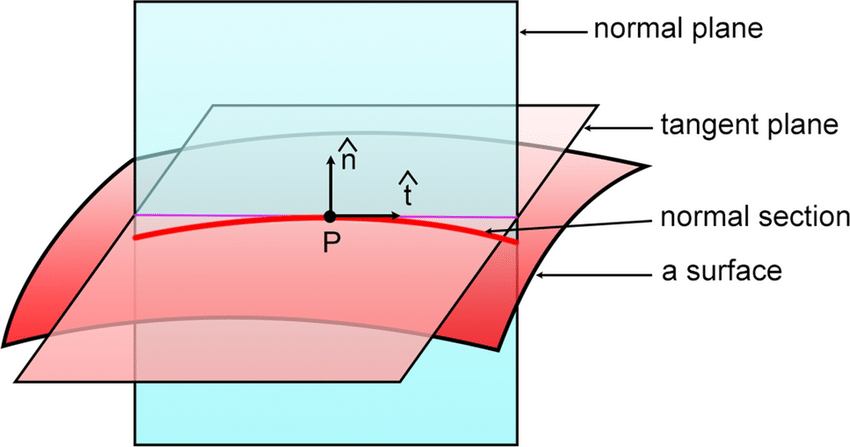
\includegraphics[width=0.5\linewidth]{Normal-section.png} % Replace 'normal_section.png' with your filename
    \caption{The normal section $\beta$ formed by the intersection of the surface $S$ and the plane spanned by the normal vector $N$ and the tangent vector $w$.}
    \label{fig:normal_section}
\end{figure}


\begin{remark}
$$ \beta''(0) = t'(0) = \kappa \mathbf{n} = k_n N + k_g T. $$
But $\beta$ obviously must lie on $\Sigma$, so $k_g = 0$.
$$ \Rightarrow k_g = \begin{cases} +\kappa & \text{if } \mathbf{n} \text{ is along the direction of } N. \\ -\kappa & \text{if } \mathbf{n} \text{ is opposite the direction of } N. \end{cases} $$
\end{remark}

\begin{proposition}
Let $\alpha: (-\varepsilon, \varepsilon) \to S$ piecewise unit speed curve (p.u.c.) with $\alpha(0) = p$ and $\alpha'(0) = w$.
Then the normal curvature of $\alpha$ on $S$ is equal to $\mathrm{II}_p(w)$.
\end{proposition}

\begin{proof}
$$ \mathrm{II}_p(w) = \langle -dN_p w, w \rangle = \langle -dN_p (\alpha'(0)), \alpha'(0) \rangle $$
$$ = - \langle (N \circ \alpha)'(0), \alpha'(0) \rangle = k_n. $$
\end{proof}

\begin{corollary}
\begin{enumerate}
    \item The normal curvature of any $\alpha: (-\varepsilon, \varepsilon) \to S$ with $\alpha'(0) = w$ are the same $\mathrm{II}_p(w)$.
    \item $\mathrm{II}_p(w)$ measures the (normal) curvature of the sectional curve of $w$.
\end{enumerate}
This gives a geometric interpretation of $\mathrm{II}_p(w)$.
\end{corollary}

\begin{corollary}
Let $w \in T_p S$ be of norm $1$. Then the curvature of the sectional curve of $w$ must lie within $\lambda_1$ and $\lambda_2$. i.e:
$$ \lambda_1 \le \mathrm{II}_p(w) \le \lambda_2 \quad \forall w \in T_p S, \quad \|w\| = 1. $$
\end{corollary}

\begin{proof}
Without loss of generality (WLOG), write $w = \cos\theta e_1 + \sin\theta e_2$, where $e_1, e_2$ principal directions of $-dN_p$ and orthogonal basis of $T_p S$.
Then:
\begin{align*}
\mathrm{II}_p(w) &= \langle\langle w, w \rangle\rangle = \langle -dN_p w, w \rangle \\
&= \langle -dN_p (\cos\theta e_1 + \sin\theta e_2), \cos\theta e_1 + \sin\theta e_2 \rangle \\
&= \lambda_1 \cos^2\theta + \lambda_2 \sin^2\theta
\end{align*}
Then we're done.
\end{proof}

\begin{remark}
Finally we can give a better geometric picture of understanding $\mathrm{II}_p$.
\end{remark}

\begin{example}

Local behavior for parabolic point $p \in S$.
$$ -\lambda \le \mathrm{II}_p(w) \le 0 \quad \text{or} \quad 0 \le \mathrm{II}_p(w) \le \lambda $$
\end{example}

\begin{remark}
\textbf{Elliptic pt:}
$$ \lambda_1 \le \mathrm{II}_p(w) \le \lambda_2. \quad \lambda_1 \lambda_2 > 0. $$
\textbf{Hyperbolic pt:}
$$ \lambda_1 \le \mathrm{II}_p(w) \le \lambda_2. \quad \lambda_1 < 0 < \lambda_2. $$
\end{remark}

\subsection{Second Fundamental Form in Local Coordinates}

\begin{remark}
\textbf{Our goal:} Find an easy way to compute $\mathrm{II}_p$ and $dN_p$.
\end{remark}

\begin{definition}
Let $N: U \to \mathbb{S}^2$ be the \textbf{normal map}.
(Recall this is actually $N \circ X$).
\end{definition}

\begin{definition}
\begin{align*}
e &= \langle -N_u, X_u \rangle. \\
f &= \langle -N_u, X_v \rangle = \langle -N_v, X_u \rangle. \\
g &= \langle -N_v, X_v \rangle.
\end{align*}
\end{definition}

\begin{proposition}
If
\begin{align*}
w_1 &= a X_u + b X_v \\
w_2 &= c X_u + d X_v
\end{align*}
then
$$ \langle\langle w_1, w_2 \rangle\rangle = \begin{pmatrix} a & b \end{pmatrix} \begin{pmatrix} e & f \\ f & g \end{pmatrix} \begin{pmatrix} c \\ d \end{pmatrix} $$
\end{proposition}

\begin{remark}
As before, we call
$$ \begin{pmatrix} e & f \\ f & g \end{pmatrix} $$
the \textbf{second fundamental form} (matrix).
\end{remark}

\begin{proof}
By straightforward calculations.
\end{proof}

\begin{remark}
$N_u, N_v$ are hard to compute, but we have $\langle N, X_u \rangle = 0$.
$$ \Rightarrow \langle N_u, X_u \rangle + \langle N, X_{uu} \rangle = 0. $$
$$ \Rightarrow \begin{cases} e = \langle N, X_{uu} \rangle \\ f = \langle N, X_{uv} \rangle \\ g = \langle N, X_{vv} \rangle \end{cases} $$
\end{remark}

\begin{example}
$$ X(u, v) = (v \cos u, v \sin u, u) \quad \text{Helicoid} $$
$$ \Rightarrow \text{f.f.f} = \mathrm{I}_p = \begin{pmatrix} E & F \\ F & G \end{pmatrix} = \begin{pmatrix} v^2+1 & 0 \\ 0 & 1 \end{pmatrix} $$
$$ N = \frac{X_u \times X_v}{\| X_u \times X_v \|} $$
Then we compute $X_{uu}, X_{uv}, X_{vv}$.
Then
\begin{align*}
e &= \langle N, X_{uu} \rangle \\
f &= \langle N, X_{uv} \rangle \\
g &= \langle N, X_{vv} \rangle
\end{align*}
$$ \Rightarrow \text{s.f.f.} = \mathrm{II}_p = \begin{pmatrix} 0 & \frac{1}{\sqrt{v^2+1}} \\ \frac{1}{\sqrt{v^2+1}} & 0 \end{pmatrix} $$
\end{example}

\begin{remark}
After understanding the second fundamental form, one can express:
$$ -dN_p: T_p S \to T_p S $$
in coordinates with $\mathcal{B} = \{ X_u, X_v \}$.

Suppose $(-dN_p)_{\mathcal{B}} = \begin{pmatrix} a_{11} & a_{12} \\ a_{21} & a_{22} \end{pmatrix}$, i.e.:
\begin{align*}
-dN_p (X_u) &= a_{11} X_u + a_{21} X_v. \\
\Rightarrow -N_u &= a_{11} X_u + a_{21} X_v. \\
-dN_p (X_v) &= a_{12} X_u + a_{22} X_v = -N_v.
\end{align*}
\begin{align*}
\Rightarrow \langle -N_u, X_u \rangle = e &= a_{11} E + a_{21} F. \\
\Rightarrow \langle -N_u, X_v \rangle = f &= a_{11} F + a_{21} G. \\
\langle -N_v, X_u \rangle = f &= a_{12} E + a_{22} F. \\
\langle -N_v, X_v \rangle = g &= a_{12} F + a_{22} G.
\end{align*}
$$ \Rightarrow \begin{pmatrix} e & f \\ f & g \end{pmatrix} = \begin{pmatrix} E & F \\ F & G \end{pmatrix} \begin{pmatrix} a_{11} & a_{12} \\ a_{21} & a_{22} \end{pmatrix} $$
$$ \Rightarrow (-dN_p)_{\mathcal{B}} = \begin{pmatrix} a_{11} & a_{12} \\ a_{21} & a_{22} \end{pmatrix} = \begin{pmatrix} E & F \\ F & G \end{pmatrix}^{-1} \begin{pmatrix} e & f \\ f & g \end{pmatrix} $$
$$ = \mathrm{I}_p^{-1} \mathrm{II}_p. $$
\end{remark}

\begin{corollary}
The Gaussian curvature $K = \frac{\det (\mathrm{II}_p)}{\det (\mathrm{I}_p)} = \frac{eg - f^2}{EG - F^2}$.
Which gives a neat formula for calculating the Gaussian curvature.
\end{corollary}

\begin{example}
Back to the previous Helicoid example.
We have $K = \det(-dN_p) = (1+v^2)^{-2}$.
$H = 0 = \frac{1}{2} \operatorname{tr}(-dN_p)$. (Example of \textbf{minimum surface}).
From here, one can easily compute the principal directions and principal curvature.
\end{example}

\begin{example}
Compute $(-dN_p)_{\mathcal{B}}$, $K$, $H$. See that $H=0$.
\end{example}

\begin{example}[Torus]
$$ X(u, v) = ((a + r \cos u) \cos v, (a + r \cos u) \sin v, r \sin u) $$
$\mathrm{I}_p$.
$\mathrm{II}_p$.
$K$.
$$ \Rightarrow K > 0 \quad \text{when} \quad -\frac{\pi}{2} < u < \frac{\pi}{2}. $$
$$ K = 0 \quad \text{when} \quad u = \frac{\pi}{2}, \frac{3\pi}{2}. $$
$$ K < 0 \quad \text{when} \quad \frac{\pi}{2} < u < \frac{3\pi}{2}. $$
\end{example}

\begin{remark}
$$ \int K dA = 0. $$
We can check this by direct calculation.
\end{remark}

\begin{exercise}
Check $H = \frac{1}{2} \cdot \frac{e G - 2 f F + g E}{E G - F^2}$.
\end{exercise}

\end{document}



